\documentclass[hidelinks,12pt,dvipsnames,border=2pt]{standalone}
%\usepackage[top=0.7in, bottom=0.8in, left=1in, right=1in]{geometry}
\usepackage{tikz}
\usepackage{hyperref}
\usetikzlibrary{arrows}
\usetikzlibrary{shapes}
\usepackage{enumitem}
\usepackage{bm}
\usepackage{mathdots}
\usepackage{amsmath}
\usepackage{tcolorbox}
\usetikzlibrary{shadings}
\usetikzlibrary{decorations.pathreplacing}
\usepackage{helvet}
\usepackage{url}
\usepackage{graphicx}
\usetikzlibrary{arrows.meta,positioning,fit,calc}
\renewcommand{\familydefault}{\sfdefault}


\usetikzlibrary{arrows,decorations.pathmorphing,backgrounds,fit,positioning,shapes.symbols,chains}

\begin{document}
	
% trim=left botm right top
\begin{tikzpicture}

\node at (0,0) {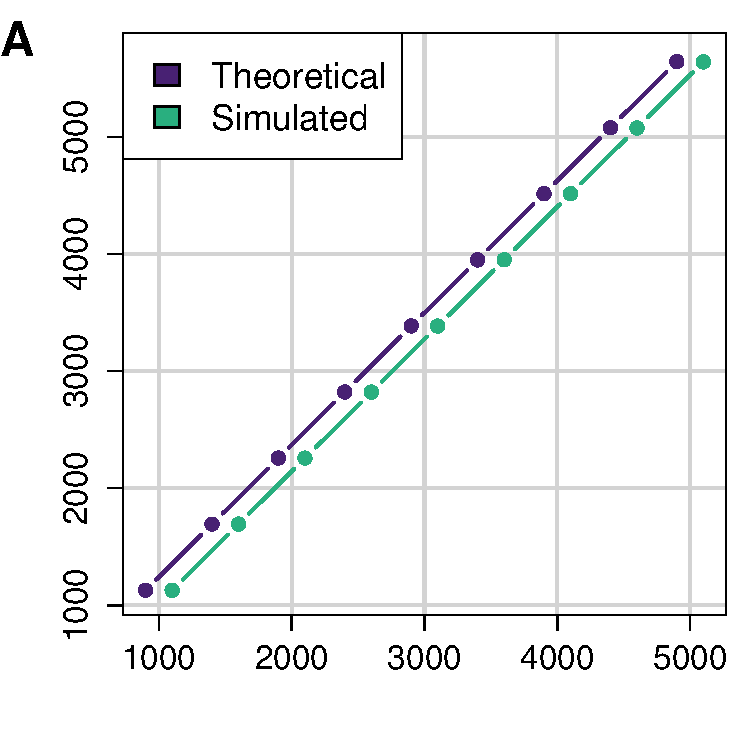
\includegraphics[width=\textwidth]{standard_normal_manhattan_sample-mean_vs_theoretical-mean.pdf}};
\node at (13.75,0) {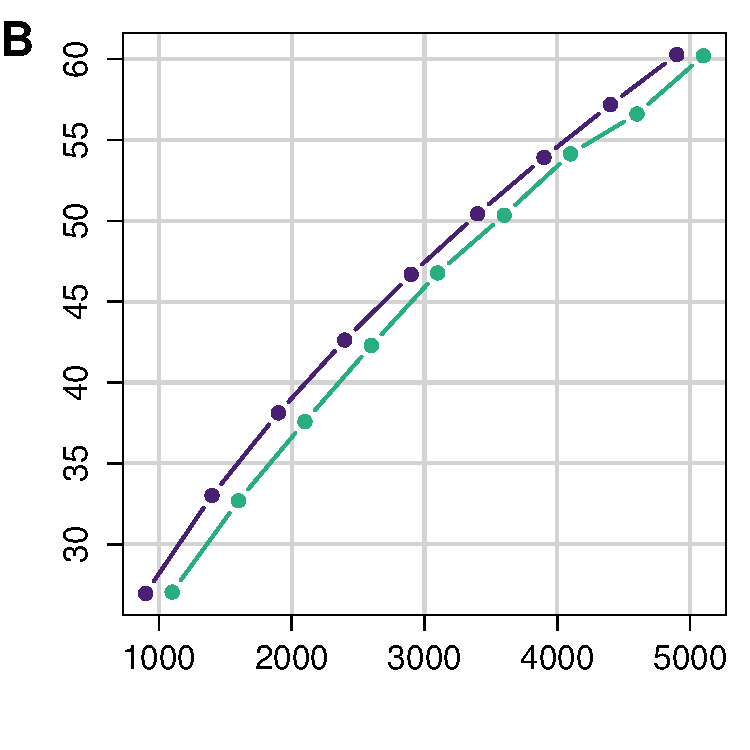
\includegraphics[width=\textwidth]{standard_normal_manhattan_sample-SD_vs_theoretical-SD.pdf}};

\node[rotate=90,xscale=1.9,yscale=1.9] at (-6.6,0.8) {Mean};
\node[rotate=90,xscale=1.9,yscale=1.9] at (7.15,0.8) {Standard Deviation};

%\node[rotate=90,xscale=1.9,yscale=1.9] at (-6.5,-11.6) {Distance (Mean $\pm$ SD)};

%\node[rotate=90,xscale=2.1,yscale=2.1] at (-7.5,-5.1) {Distance (Mean $\pm$ SD)};

\node[xscale=1.9,yscale=1.9] at (7.95,-6.3) {Number of Attributes ($p$)};

\node[xscale=1.9,yscale=1.9] at (7.95,7.5) {Moments of Manhattan Distances in Standard Normal Data};

\end{tikzpicture}

\end{document}